
\renewcommand{\stage}{1. Learning a policy}
% 22 frames, 25 minutes
\begin{frame}{1. Actor--critic methods}
\begin{columns}[c]
\column{.52\textwidth}
{\Large Actor-Critics Can Achieve Optimal Sample Efficiency}\gap
Joint work: Kevin Tan, Wei Fan, Yuting Wei.\gap ICML 2025
\column{.44\textwidth}
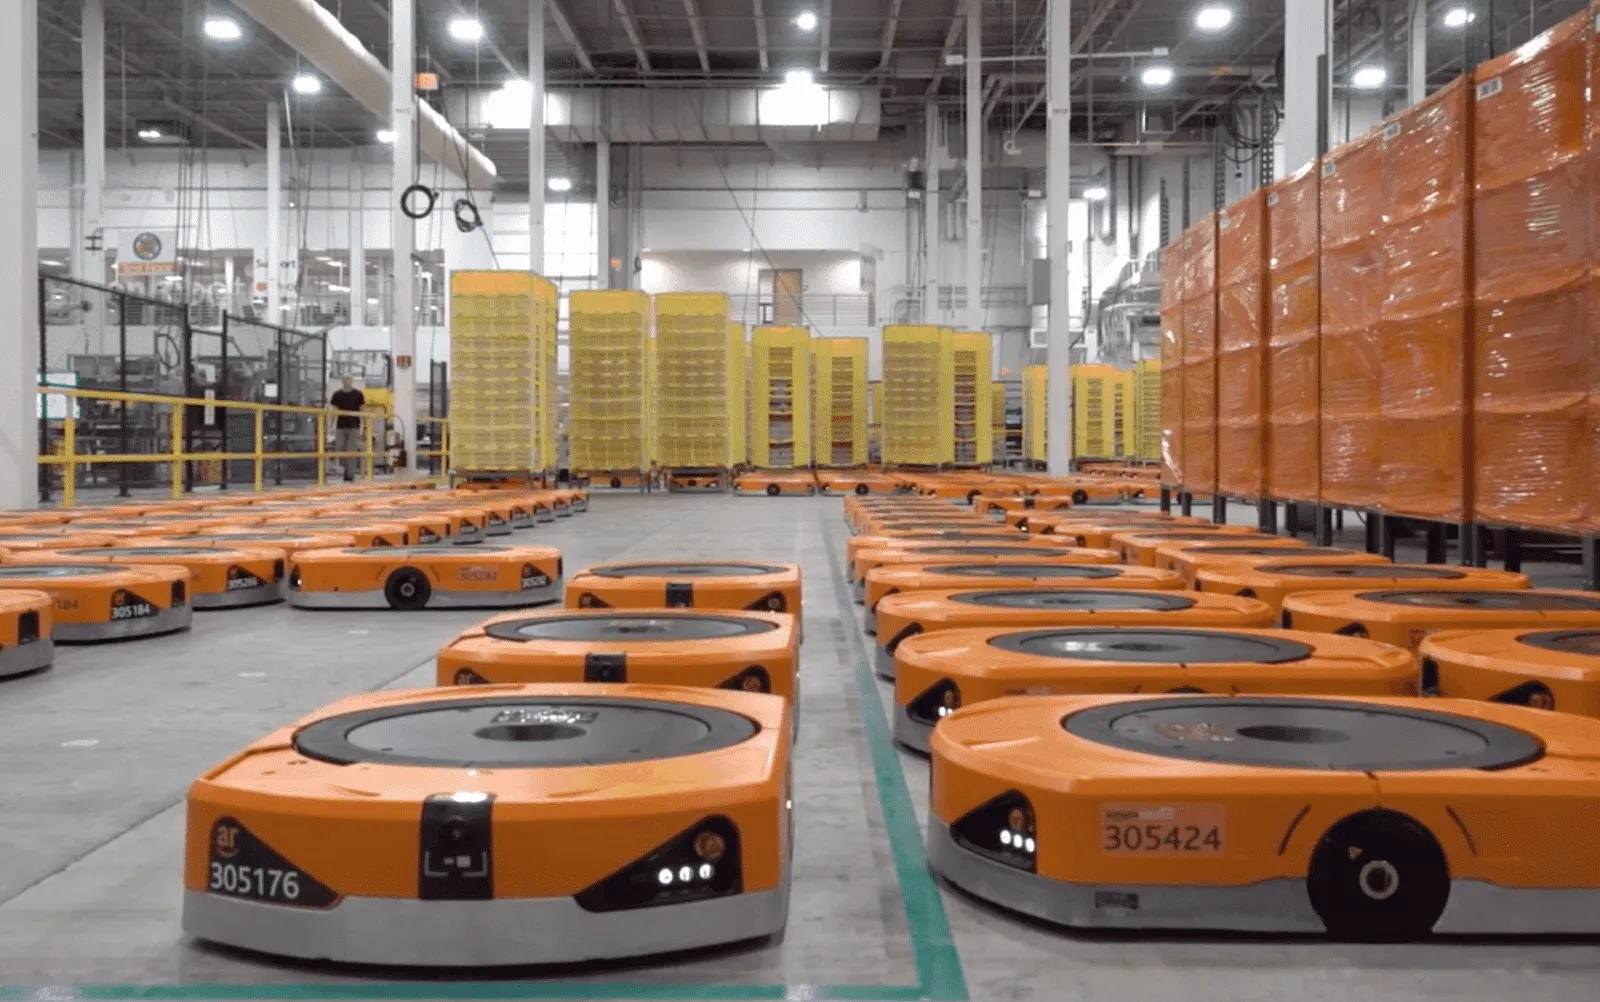
\includegraphics[width=\linewidth]{section-warehouse.png}
\end{columns}
\gap Can an actor--critic learn efficiently when it has to explore?
\end{frame}

\begin{frame}{Actions affect later rewards}
\begin{center}\begin{tikzpicture}[x=1cm,y=1cm]
\path[use as bounding box] (0,0) rectangle (12,4.6);
\node[obj] (s) at (1.5,3.5) {$s_h$};\node[lab,above=3mm of s] {Position, velocity};
\node[obj] (a) at (5.5,3.5) {$a_h$};\node[lab,above=3mm of a] {Motor command};
\node[obj] (sn) at (10,3.5) {$s_{h+1}$};\node[lab,above=3mm of sn] {Next state};
\draw[arr] (s)--node[above,lab]{policy $\pi_h$}(a);
\draw[arr] (a)--node[above,lab]{dynamics}(sn);
\node[lab,text=green] at (8,2.7) {Reward $r_h\in[0,1]$};
\begin{scope}[visible on=<2->]
\node at (6,1.7) {$\pi_h(a\mid s)=\Pr(a_h=a\mid s_h=s)$};
\draw[arr] (.4,.5)--(11.7,.5);
\foreach \x/\t in {1/1,3/2,5/3,10.7/H}{\draw (\x,.4)--(\x,.6);\node[lab,below] at (\x,.35) {step $\t$};}
\node at (7.8,.8) {$\cdots$};
\end{scope}
\end{tikzpicture}\end{center}
\uncover<3->{One episode: $H$ decisions. Goal: maximize $\E[\sum_{h=1}^H r_h]$.}
\src{Finite action set $\A$.}
\end{frame}

\begin{frame}{Estimating total reward}
\begin{center}\begin{tikzpicture}[x=1cm,y=1cm]
\path[use as bounding box] (0,0) rectangle (12,3.2);
\node[obj] (s) at (1,2.1) {$s$};\node[obj] (a) at (3,2.1) {$a$};
\node[obj] (sp) at (5.3,2.1) {$s'$};
\draw[arr] (s)--node[above,lab]{choose}(a);
\draw[arr] (a)--node[above,lab]{$r_h$}(sp);
\draw[arr] (sp)--(11,2.1);
\foreach \x/\r in {7/r_{h+1},9/r_{h+2},11/r_H}{\fill[blue] (\x,2.1) circle (2pt);\node[above,lab] at (\x,2.3) {$\r$};}
\node[lab] at (8.3,1.3) {Follow $\pi$ for remaining steps};
\draw[decorate,decoration={brace,mirror,amplitude=5pt}] (2.7,.8)--(11.4,.8);
\node at (7,.2) {$Q_h^\pi(s,a)$};
\end{tikzpicture}\end{center}
\[
Q_h^\pi(s,a)=\E\!\left[\sum_{k=h}^{H}r_k\;\middle|\;s_h=s,a_h=a,\text{ then }\pi\right].
\]
\pause
\[
V_h^\pi(s)=\underbrace{\sum_{a\in\A}\pi_h(a\mid s)Q_h^\pi(s,a)}_{\text{average over the first action}}.
\]
\end{frame}

\begin{frame}{What is an actor--critic?}
\begin{center}\begin{tikzpicture}[x=1cm,y=1cm]
\path[use as bounding box] (0,-.1) rectangle (12,5.3);
\node[text=blue,font=\large] at (2,4.9) {Critic};
\node[text=pink,font=\large] at (9.5,4.9) {Actor};
\draw[arr] (.5,2.8)--(.5,4.4);\draw[arr] (.5,2.8)--(3.7,2.8);
\draw[blue,thick] (.7,3.0)--(3.4,4.2);
\foreach \x/\y in {1/3.2,1.5/3.25,2/3.7,2.7/3.8,3.2/4.15}{\fill[black!60] (\x,\y) circle(2pt);}
\node[lab] at (2,2.25) {Inputs $(s,a)$};\node[rotate=90,lab] at (.05,3.6) {Value $f_h$};
\draw[arr] (7.6,2.8)--(11.5,2.8);
\foreach \x/\h/\a in {8/.6/a_1,9.4/1.4/a_2,10.8/.9/a_3}{\draw[fill=pink!25,draw=pink] (\x-.3,2.8) rectangle (\x+.3,2.8+\h);\node[lab,below] at (\x,2.8) {$\a$};}
\node[lab] at (9.5,2.05) {Policy $\pi_h(a\mid s)$};\node[rotate=90,lab] at (7.2,3.6) {Probability};
\draw[arr,visible on=<2->] (3.8,3.7)--node[above,lab]{estimated values}(6.9,3.7);
\draw[arr,visible on=<3->] (9.5,1.7)--(9.5,.8)--node[below,lab]{new transitions $(s,a,r,s')$}(2,.8)--(2,1.7);
\end{tikzpicture}\end{center}
\uncover<2->{Higher estimated value raises an action's odds.}

\end{frame}

\begin{frame}{The critic update is a regression problem}
\begin{center}\begin{tikzpicture}[x=1cm,y=1cm]
\path[use as bounding box] (0,0) rectangle (12,3.6);
\node[anchor=west] at (0,3.3) {Observed transition: $(s,a,r,s')$};
\node[obj] (r) at (1,2) {$r$};\node[lab,above=2mm of r] {Observed reward};
\node[obj] (sp) at (4,2) {$s'$};
\node (next) at (8,2) {$\sum_b\pi_{h+1}(b\mid s')f_{h+1}(s',b)$};
\draw[arr] (sp)--(next);\node[lab,above=2mm of next] {Estimated remaining reward};
\draw[arr,visible on=<2->] (r.south)--(1,.35)--(5.5,.35);
\draw[arr,visible on=<2->] (next.south)--(8,.35)--(6.5,.35);
\node[visible on=<2->] at (6,.35) {$y$};
\end{tikzpicture}\end{center}
\uncover<2->{\[
y=r+\sum_b\pi_{h+1}(b\mid s')f_{h+1}(s',b).
\]}
\uncover<3->{\[
\widehat f_h\in\arg\min_{f_h\in\F_h}\sum_{(s,a,r,s')\in D_h}(f_h(s,a)-y)^2.
\]}
\uncover<3->{$D_h$: transitions at step $h$. $\F_h$: regression class.}
\end{frame}

\begin{frame}{Updating the policy}
\begin{center}\begin{tikzpicture}[x=1cm,y=1cm]
\path[use as bounding box] (0,0) rectangle (12,2.8);
\node at (1.4,2.2) {$\pi_{t,h}(a\mid s)$};
\node at (5.8,2.2) {$\pi_{t,h}(a\mid s)e^{\eta f_{t,h}(s,a)}$};
\node at (10.5,2.2) {$\pi_{t+1,h}(a\mid s)$};
\draw[arr] (2.7,2.2)--node[above,lab]{reweight}(3.6,2.2);
\draw[arr,visible on=<2->] (8.1,2.2)--node[above,lab]{normalize}(9.1,2.2);
\node[lab] at (1.4,1.2) {Old probabilities};
\node[lab] at (5.8,1.2) {$\eta>0$: learning rate\\$t$: episode index};
\node[lab,visible on=<2->] at (10.5,1.2) {Sum to one};
\end{tikzpicture}\end{center}
\uncover<2->{\[
\pi_{t+1,h}(a\mid s)=\frac{\pi_{t,h}(a\mid s)e^{\eta f_{t,h}(s,a)}}{\sum_{b\in\A}\pi_{t,h}(b\mid s)e^{\eta f_{t,h}(s,b)}}.
\]}
\uncover<3->{\[
\underbrace{\frac{\pi_{t+1,h}(a\mid s)}{\pi_{t+1,h}(b\mid s)}}_{\text{new odds}}
=\underbrace{\frac{\pi_{t,h}(a\mid s)}{\pi_{t,h}(b\mid s)}}_{\text{old odds}}
e^{\eta\underbrace{[f_{t,h}(s,a)-f_{t,h}(s,b)]}_{\text{estimated advantage}}}.
\]}
\end{frame}

\begin{frame}{Exploring rarely tried actions}
\begin{center}\begin{tikzpicture}[x=1cm,y=1cm]
\path[use as bounding box] (0,0) rectangle (12,3.6);
\node[obj,circle] (s) at (1,1.8) {$s$};
\node[lab] (a) at (4,2.8) {Often visited};\node[lab] (b) at (4,.8) {Rarely visited};
\draw[arr] (s)--(a);\draw[arr,dashed] (s)--(b);
\draw[blue,very thick] (7.2,2.8)--(8.1,2.8);\fill[blue] (7.65,2.8) circle(2pt);
\draw[blue,very thick] (6.5,.8)--(10.5,.8);\fill[blue] (8.5,.8) circle(2pt);
\foreach \x/\y in {7.2/2.8,8.1/2.8,6.5/.8,10.5/.8}{\draw[blue] (\x,\y-.15)--(\x,\y+.15);}
\node[lab] at (8.5,3.4) {Values allowed by the data};
\node[lab] at (8.5,.05) {Wider uncertainty};
\draw[arr,pink,visible on=<2->] (11.5,1.4)--(10.5,.85);
\node[lab,text=pink,visible on=<2->] at (11.2,2) {Use upper\\endpoint};
\end{tikzpicture}\end{center}
\uncover<2->{\[
f_h(s,a)=\sup_{q\in\mathcal C}q_h(s,a),\qquad
\mathcal C=\{\text{critics consistent with Bellman regression data}\}.
\]}
\uncover<3->{Alg. 1: policy-evaluation target $+$ pointwise optimism $+$ softmax update.}
\src{Illustrative intervals.}
\end{frame}

\begin{frame}{How much reward do we lose while learning?}
\begin{center}\begin{tikzpicture}[x=1cm,y=1cm]
\path[use as bounding box] (0,0) rectangle (12,2.6);
\foreach \x/\t/\v in {2/1/.7,5/2/1.1,8/3/1.5,11/T/1.8}{
\draw[green,thick] (\x-.5,2.2)--(\x+.5,2.2);
\draw[blue,thick] (\x-.5,\v)--(\x+.5,\v);
\draw[<->,pink] (\x,\v+.05)--(\x,2.15);
\node[lab] at (\x,.25) {episode $\t$};}
\node[text=green,anchor=west,lab] at (0,2.6) {Optimal value $V_1^{\pi^*}(s_1)$};
\node[text=blue,anchor=west,lab] at (0,-.3) {Current value $V_1^{\pi_t}(s_1)$};
\end{tikzpicture}\end{center}
\[
\Reg(T)=\sum_{t=1}^T\underbrace{[V_1^{\pi^*}(s_1)-V_1^{\pi_t}(s_1)]}_{\text{reward lost in episode }t}.
\]
\pause
\[
\Reg(T)=\widetilde O(\sqrt T)\quad\Longrightarrow\quad
\frac{\Reg(T)}{T}=\widetilde O(T^{-1/2}).
\]
Fixed starting state $s_1$.
\src{$\widetilde O$ hides logarithms. The rate also depends on $H$ and model complexity.}
\end{frame}

\begin{frame}{The regression response depends on past critics}
From a uniform initial policy,
\[
\pi_{t+1,h}(a\mid s)\propto\exp\!\left\{\eta\sum_{\tau=1}^{t}f_{\tau,h}(s,a)\right\}.
\]
\begin{center}\begin{tikzpicture}[x=1cm,y=0.78cm]
\path[use as bounding box] (0,0) rectangle (12,3.2);
\foreach \x/\i in {1/1,3/2,6/t}{\node[obj] (q\i) at (\x,2.6) {$f_{\i}$};\draw[arr] (q\i.south)--(4,1.3);}
\node at (4.5,2.6) {$\cdots$};
\node (sum) at (4,1) {$\sum_{\tau\leq t} f_\tau$};
\node (pi) at (9.5,1) {$\pi_{t+1}$};
\draw[arr] (5,1)--(8.8,1);\node[lab] at (6.9,1.45) {softmax};
\end{tikzpicture}\end{center}
\uncover<2->{\[
y=r+\sum_b\underbrace{\pi_{t+1}(b\mid s')}_{\text{depends on past critics}}f(s',b).
\]}
\uncover<3->{Reusing the data requires a uniform bound over these responses.}
\end{frame}

\begin{frame}{How complicated is a sum of critics?}
\begin{columns}[T,onlytextwidth]
\column{.47\textwidth}
\textbf{Unclipped linear critics}\par\medskip
Shared features $x$, coefficients $w_t$:
\[
\sum_{t=1}^T x^\top w_t
=x^\top\underbrace{\Big(\sum_{t=1}^T w_t\Big)}_{\text{one vector}}.
\]
\column{.50\textwidth}
\uncover<2->{\textbf{Hinge critics}\par\medskip
$f_u(x)=\max(0,x-u)$\par\smallskip
\centering\begin{tikzpicture}[x=4.7cm,y=1.75cm,font=\scriptsize]
\draw[arr] (0,0)--(1.06,0) node[right] {$x$};
\draw[arr] (0,0)--(0,1.13) node[above] {value};
\draw[blue,dashed,thick] (0,0)--(.25,0)--(1,.75);
\draw[green,dotted,very thick] (0,0)--(.75,0)--(1,.25);
\draw[pink,thick] (0,0)--(.25,0)--(.75,.5)--(1,1);
\foreach \x/\txt in {.25/{.25},.75/{.75},1/1}{\draw (\x,0)--(\x,-.05) node[below] {$\txt$};}
\foreach \y in {.5,1}{\draw (0,\y)--(-.02,\y) node[left] {$\y$};}
\draw[blue,dashed,thick] (.09,1)--(.21,1);\node[anchor=west] at (.22,1) {$f_{.25}$};
\draw[green,dotted,very thick] (.09,.79)--(.21,.79);\node[anchor=west] at (.22,.79) {$f_{.75}$};
\draw[pink,thick] (.09,.58)--(.21,.58);\node[anchor=west] at (.22,.58) {sum};
\end{tikzpicture}\par
Each new threshold adds a bend.}
\end{columns}
\uncover<3->{\gap $M$ approximations per fit, $K$ fits $\ \Longrightarrow\ $ up to $M^K$ sequences.
\[
K=T\quad\Longrightarrow\quad
\underbrace{\sqrt{T\log(M^T)}}_{\text{regret term}}=T\sqrt{\log M}.
\]}
\end{frame}

\begin{frame}{Can we update the critic less often?}
\begin{center}\begin{tikzpicture}[x=1cm,y=.8cm]
\path[use as bounding box] (0,0) rectangle (12,4.5);
\draw[arr] (.5,3.5)--(11.6,3.5) node[right] {$t$};
\foreach \x/\i in {1/1,5/2,9/3}{\draw[pink,very thick] (\x,3.2)--(\x,3.9);\node[above,lab] at (\x,3.9) {critic $\i$};}
\foreach \x in {1.6,2.4,...,10.4}{\draw[arr,blue] (\x,2.8)--(\x+.45,2.8);}
\node[lab] at (6,2.2) {Actor changes every episode};
\begin{scope}[visible on=<2->]
\node at (2,1) {$f_{h+1}\ \text{fixed}$};
\node at (6,1) {$\pi_t\ \text{changes}$};
\node at (10,1) {$y_t^\pi\ \text{changes}$};
\draw[arr] (3.5,1)--(4.4,1);\draw[arr] (7.5,1)--(8.5,1);
\end{scope}
\end{tikzpicture}\end{center}
\uncover<2->{\[y_t^\pi=r+\sum_b\pi_t(b\mid s')f_{h+1}(s',b).\]}
\uncover<2->{$\mathcal T_h^{\pi_t}f_{h+1}=\E[y_t^\pi\mid s,a]$: expected regression response.\par}\medskip
\uncover<3->{Between critic updates, does the old upper bound still hold?}
\end{frame}

\begin{frame}{When does the old critic stop being optimistic?}
Zero reward. One next state $s'$ with action values $(0,1)$.
\[p=\pi(a_2\mid s'),\qquad y^\pi=(1-p)\,0+p\,1=p.\]
\begin{center}\begin{tikzpicture}[x=.96cm,y=1cm]
\draw[arr] (0,0)--(11,0) node[right,lab]{value};
\foreach \x/\v in {0/0,2/.2,4/.4,8/.8,10/1}{\draw (\x,-.07)--(\x,.07);\node[below,lab] at (\x,-.1) {$\v$};}
\draw[blue,thick] (2,.15)--(2,.8);\node[above,lab,text=blue] at (2,.82) {Old target};
\draw[pink,very thick] (4,-.1)--(4,1.65);\node[above,lab,text=pink] at (4,1.65) {Fixed critic $f_h(s,a)$};
\begin{scope}[visible on=<2->]
\draw[arr,blue,thick] (2,.37)--(8,.37);\draw[blue,thick] (8,.14)--(8,.8);\node[above,lab,text=blue] at (8,.82) {New target};
\end{scope}
\end{tikzpicture}\end{center}
\uncover<3->{The shortfall is $.8-.4=.4$ each episode this gap persists.}
\end{frame}

\begin{frame}{Use an optimality target instead}

\begin{center}\renewcommand{\arraystretch}{1.5}
\begin{tabular}{lcc}
\toprule
Probability of $a_2$ & Evaluation target & \uncover<2->{Optimality target}\\
\midrule
$.2$ & $.8(0)+.2(1)=.2$ & \uncover<2->{$\max(0,1)=1$}\\
$.8$ & $.2(0)+.8(1)=.8$ & \uncover<2->{$\max(0,1)=1$}\\
\bottomrule
\end{tabular}\end{center}
\uncover<2->{Regression target $r+\max_b f(s',b)$, independent of the actor.}
\uncover<3->{\[
|\max_b f(s',b)-\max_b g(s',b)|\leq\|f-g\|_\infty .
\]}
\uncover<3->{The same cover works for the maxima.}
\end{frame}

\begin{frame}{Optimism holds as the actor changes}
$\T_h f$: expected optimality target. $\T_h^\pi f$: expected policy-evaluation target.\\On the confidence event:
\begin{center}\begin{tikzpicture}[x=1cm,y=0.87cm]
\path[use as bounding box] (0,0) rectangle (12,4.5);
\draw[arr] (1,.4)--(1,4.2) node[above,lab]{Value at $(s,a)$};
\draw[pink,thick] (2,3.7)--(10.5,3.7);\node[right] at (10.5,3.7) {$f_h$};
\draw[green,thick,visible on=<2->] (2,2.6)--(10.5,2.6);\node[right,visible on=<2->] at (10.5,2.6) {$\T_h f_{h+1}$};
\foreach \x/\y/\polindex in {3/1.1/t,6/1.8/{t+1},9/1.4/{t+2}}{
\fill[blue,visible on=<3->] (\x,\y) circle(3pt);
\node[below,lab,visible on=<3->] at (\x,\y-.1) {$\T_h^{\pi_{\polindex}} f_{h+1}$};}
\node[lab,text=pink] at (6,4.1) {Optimistic critic};
\node[lab,text=green,visible on=<2->] at (6,3) {Best next action};
\end{tikzpicture}\end{center}
\uncover<3->{\[f_h\geq\T_h f_{h+1}\geq\T_h^{\pi_t}f_{h+1}\qquad\text{for every actor }\pi_t.\]}
\src{At each $(s,a)$, a policy average is at most the maximum.}
\end{frame}

\begin{frame}{The actor must track the greedy policy}
Tracking error at $\pi(a_2\mid s')=.8$:
\[
\max_a f(s',a)-\sum_a\pi(a\mid s')f(s',a)=1-.8=.2 .
\]
\begin{center}\begin{tikzpicture}[x=1cm,y=.80cm]
\path[use as bounding box] (0,0) rectangle (12,4.1);
\foreach \x/\lab in {2/Before reset,6/Reset,10/After softmax updates}{\node[lab] at (\x,3.8) {\lab};\draw[arr] (\x-1.2,1)--(\x+1.2,1);}
\draw[fill=blue!20,draw=blue] (.9,1) rectangle (1.6,2.92);\draw[fill=pink!20,draw=pink] (2.2,1) rectangle (2.9,1.48);
\foreach \x in {4.9,6.2}{\draw[fill=black!10] (\x,1) rectangle (\x+.7,2.2);}
\draw[fill=blue!20,draw=blue] (8.9,1) rectangle (9.6,1.48);\draw[fill=pink!20,draw=pink] (10.2,1) rectangle (10.9,2.92);
\foreach \x in {2,6,10}{\node[lab] at (\x-.75,.6) {$a_1$};\node[lab] at (\x+.6,.6) {$a_2$};}
\draw[arr] (3.4,2.2)--(4.4,2.2);\draw[arr] (7.4,2.2)--(8.4,2.2);
\node[lab,text=pink] at (2,0) {New critic favors $a_2$};
\node[lab] at (6,0) {$\pi(a\mid s)=1/|\A|$};
\node[lab] at (10,0) {Probability of $a_2$: $.8$};
\end{tikzpicture}\end{center}
\pause
\[
\pi(a^*\mid s)=\varepsilon\ \Rightarrow\ \KL(\pi^f\|\pi)=\log(1/\varepsilon),\qquad
\text{after reset: }\log|\A|.
\]
{\small Bars: action probabilities. $a^*$: new greedy action. $\pi^f$: policy choosing it.}
\end{frame}

\begin{frame}{Alg. 2: update the critic when its regression error grows}
On retained step-$h$ transitions $D_{t,h}$,
\[
L_{t,h}(q,f)=\sum_{(s,a,r,s')\in D_{t,h}}[q(s,a)-r-\max_b f_{h+1}(s',b)]^2.
\]
\uncover<2->{\[
\Delta_h=\underbrace{L_{t,h}(f_h,f)}_{\text{current critic}}-
\underbrace{\min_{q\in\F_h}L_{t,h}(q,f)}_{\text{refit in the critic class}}.
\]}
\begin{center}\begin{tikzpicture}[x=1cm,y=0.75cm]
\path[use as bounding box] (0,0) rectangle (12,2.5);
\node[visible on=<2->] (test) at (6,2) {$\Delta_h\geq5H^2\beta$ for any $h$?};
\node[align=center,visible on=<3->] (keep) at (2,.6) {Keep critic\\Continue softmax updates};
\node[align=center,visible on=<3->] (new) at (9.8,.6) {Refit confidence set\\New optimistic critic; reset actor};
\draw[arr,visible on=<3->] (test.west)-|node[above,pos=.3,lab]{no}(keep.north);
\draw[arr,visible on=<3->] (test.east)-|node[above,pos=.3,lab]{yes}(new.north);
\end{tikzpicture}\end{center}
\uncover<2->{$\beta$: confidence threshold.}\par\uncover<3->{Refit cutoff: excess loss $\le H^2\beta$ at every step.}

\end{frame}

\begin{frame}{Rare critic changes limit the cost of resets}
$d$ measures how often new data reveal a previously undetected Bellman error.
\begin{center}\begin{tikzpicture}[x=1cm,y=1cm]
\path[use as bounding box] (0,0) rectangle (12,1.5);
\draw[arr] (.5,.6)--(11.5,.6);
\foreach \x/\lab in {1/t_1,4/t_2,8/t_3}{\draw[pink,very thick] (\x,.3)--(\x,.9);\node[above,lab] at (\x,.9) {$\lab$: reset};}
\node[lab] at (6,0) {The regression test triggers $K=O(dH\log T)$ changes};
\end{tikzpicture}\end{center}
\uncover<2->{\[
\underbrace{\eta H^3T}_{\text{softmax update error}}+
\underbrace{\frac{2KH\log|\A|}{\eta}}_{\text{relearning after resets}}+
\underbrace{6KH^2}_{\text{switch cost}}.
\]}
\uncover<3->{\[
\eta\asymp\sqrt{\frac{d\log T\log|\A|}{HT}}
\quad\Longrightarrow\quad\text{tracking cost}=\widetilde O(\sqrt{dH^5T}+dH^3).
\]}

\src{$d$: Dirac-type Bellman eluder dimension at scale $T^{-1/2}$.}
\end{frame}

\begin{frame}{Regret guarantee}
Critics are bounded by $H$. Assume:
\begin{center}\begin{tikzpicture}[x=1cm,y=1cm]
\path[use as bounding box] (0,0) rectangle (12,1.8);
\node at (2,1.5) {$Q^*\in\F$};\node[lab] at (2,.7) {Optimal value\\representable};
\node at (6,1.5) {$\T\F\subseteq\mathcal G$};\node[lab] at (6,.7) {Expected targets\\representable in $\mathcal G$};
\node at (10,1.5) {$d,\ \log\mathcal N$};\node[lab] at (10,.7) {Controlled sequential\\and covering complexity};
\end{tikzpicture}\end{center}
\uncover<2->{With probability at least $1-\delta$,}
\uncover<2->{\[
\Reg(T)=\widetilde O\!\left(
\underbrace{\sqrt{dH^5T\log|\A|}+dH^3}_{\text{actor tracking and switches}}
+\underbrace{\sqrt{dH^4T\log\mathcal N}}_{\text{critic error}}\right).
\]}
\uncover<2->{$\mathcal N$: covering number of critics and expected optimality targets at scale $1/T$.}
\uncover<3->{\gap $\sqrt T$ dependence for controlled complexity.\\Computing the confidence set can be expensive.}
\src{$\mathcal G$: auxiliary regression class. Logarithms in $H,T,1/\delta$ suppressed.}
\end{frame}

\begin{frame}{Online experiment: Tetris}
\begin{center}\begin{tikzpicture}
\node[inner sep=0] (p) {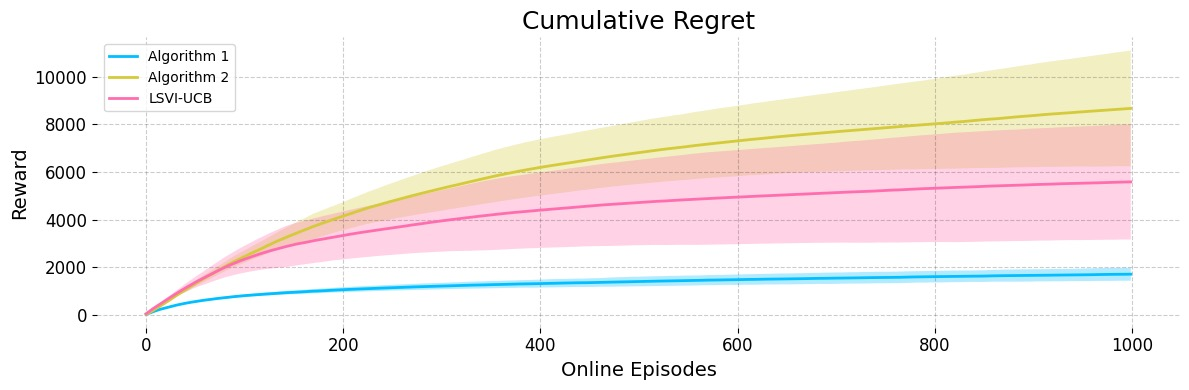
\includegraphics[width=12.6cm]{actor-regret.jpg}};
% Source's y-axis says Reward despite the plot and manuscript describing cumulative regret.
\fill[white] (p.south west) rectangle ($(p.south west)+(.37,4.13)$);
\node[rotate=90,font=\small] at ($(p.south west)+(.15,2.1)$) {Cumulative regret};
\end{tikzpicture}\end{center}
Alg. 1 has the lowest regret (30 trials).
\pause\gap
Tetris uses unclipped linear critics. Their sum still fits in one vector.
\src{Both use exploration bonuses. LSVI-UCB: optimistic value iteration. Band statistic unspecified.}
\end{frame}

\begin{frame}{When can Alg. 2 learn without optimism?}
\begin{center}\begin{tikzpicture}[x=1cm,y=.65cm]
\path[use as bounding box] (0,0) rectangle (12,4.2);
\node[lab] at (2,3.9) {Offline transitions};\node[lab] at (2,1.3) {Online transitions};
\foreach \x/\y in {.9/3.4,1.5/3.1,2.1/3.5,2.8/3.2,3.2/3.6}{\fill[green] (\x,\y) circle(2pt);}
\foreach \x in {1,2,3}{\fill[blue] (\x,.6) circle(2pt);}\draw[arr,blue] (1,.6)--(3.5,.6);
\node (fit) at (6.2,2.4) {$\widehat f\in\arg\min L(f)$};\node[lab] at (6.2,3.2) {Bellman regression};
\node (actor) at (10.5,2.4) {$\pi_{t+1}$};\node[lab] at (10.5,3.2) {Softmax update};
\draw[arr] (3.5,3.3)--(fit);\draw[arr] (3.5,.7)--(fit);\draw[arr] (fit)--(actor);
\end{tikzpicture}\end{center}
\uncover<2->{\[
\text{Offline squared Bellman error}
\ \xrightarrow{\ \text{coverage}\ }\ 
\text{Bellman error under }\pi^*.
\]}
\uncover<3->{Alg. 2 with optimality targets and $N_{\rm off}$ offline samples:
\[
\text{Additional regret}
=O\!\left(\sqrt{\beta^* H^4 c_{\rm off}^*T^2/N_{\rm off}}\right).
\]
Bounded coverage coefficient $c_{\rm off}^*$ and $N_{\rm off}=\Omega(T)$ preserve the $\widetilde O(\sqrt T)$ rate under Alg. 2's complexity assumptions.}
\src{$\beta^*$: confidence width for optimality targets. Policy evaluation also requires a policy cover.}
\end{frame}

\begin{frame}{AntMaze: a neural implementation comparison}
\begin{columns}[c]
\column{.65\textwidth}
\begin{tikzpicture}
\node[inner sep=0] (p) {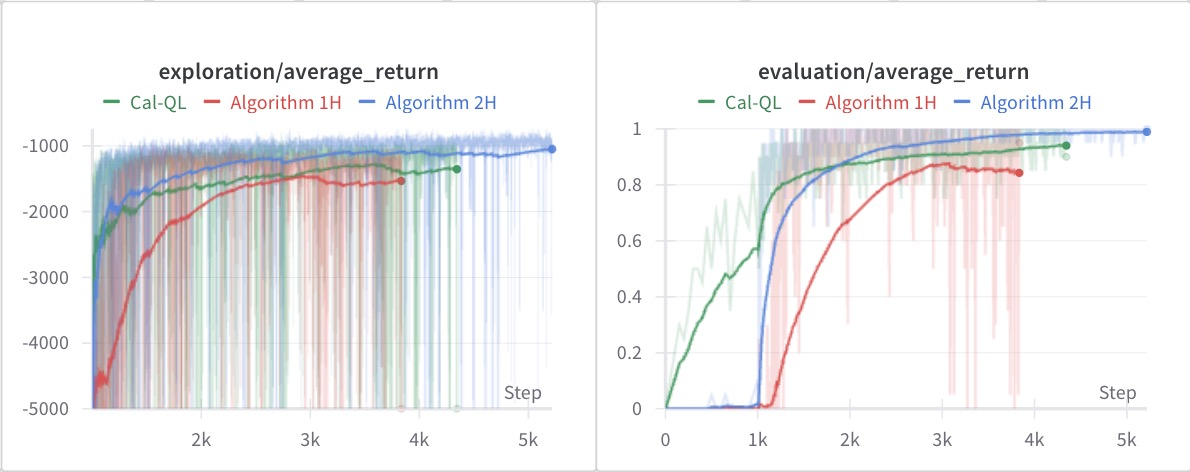
\includegraphics[width=.94\linewidth,trim=610bp 15bp 25bp 85bp,clip]{actor-hybrid.jpg}};
\node[rotate=90,font=\small] at ($(p.west)+(-.3,0)$) {Evaluation return};
\end{tikzpicture}
\column{.33\textwidth}
\textcolor{blue}{Alg. 2H}: maximum over 10 sampled actions; no resets.\gap
\textcolor{red}{Alg. 1H}: policy-evaluation target.\gap
\textcolor{green}{Cal-QL}: hybrid RL baseline.
\end{columns}
\pause\gap
Alg. 2H reaches the highest return here.
\src{AntMaze medium-diverse-v2. First 1,000 training steps: offline pretraining. Curves exponentially smoothed. ICML 2025.}
\end{frame}

\begin{frame}{Actor--critic: optimality targets and policy resets}
\begin{center}\begin{tikzpicture}[x=1cm,y=1cm]
\path[use as bounding box] (0,0) rectangle (12,5.1);
\node[anchor=west,text=blue,font=\large] at (0,4.8) {Critic};
\node at (3,3.8) {$r+\sum_a\pi(a\mid s')f(s',a)$};
\node at (9.5,3.8) {$r+\max_a f(s',a)$};
\draw[arr] (5.8,3.8)--(7.4,3.8);
\node[lab] at (9.5,2.9) {No growing policy cover};
\begin{scope}[visible on=<2->]
\node[anchor=west,text=pink,font=\large] at (0,2) {Actor};
\draw[arr] (2.2,1.2)--(11.4,1.2);
\foreach \x in {3,7.3}{\draw[pink,very thick] (\x,.9)--(\x,1.6);\node[above,lab] at (\x,1.6) {reset to uniform};}
\foreach \x in {3.5,4.2,...,10.5}{\fill[blue] (\x,1.2) circle(1.8pt);}
\node[lab] at (7,.5) {Softmax steps; rare critic changes};
\end{scope}
\end{tikzpicture}\end{center}
\uncover<3->{Next, how do we fit a model when the state is hidden?}
\end{frame}
